\documentclass[10pt,twocolumn]{article}

\usepackage{fullpage}
\usepackage{graphicx} 

\newcommand{\figref}[1]{Fig.~\ref{#1}}
\newcommand{\mypara}{\vspace{6pt}\noindent}
\newcommand{\sonet}{{SONet}}

\begin{document}

%\title{SONet (Scientific Observations Network): Facilitating Data
%  Interoperability within the Environmental and Ecological Sciences}

\title{\textbf{\sonet: A Scientific Observations Network for
    Environmental and Ecological Data Interoperability}}

\author{Mark Schildhauer$^1$, Shawn Bowers$^2$, Josh Madin$^4$,
  Corinna Gries$^3$, Deborah McGuinness$^5$, \\
  Matt Jones$^1$, Phillip Dibner$^6$, Luis
  Bermudez$^7$, John Graybeal$^7$ \\[12pt]
  $^1$NCEAS, UC Santa Barbara, $^2$UC Davis Genome Center,
  $^3$CAP/LTER and \\ Arizona State University, $^4$Macquarie
  University, Australia, $^5$McGuinness \\ Associates, $^6$Open
  Geospatial Consortium Interoperability Institute, $^7$Monterey \\
  Bay Aquarium Research Institute}

\date{September, 8, 2008}


\maketitle

\thispagestyle{empty}


\mypara Advances in ecological, biodiversity, and other environmental
and life sciences increasingly depend on the use of information from
multiple disciplines to tackle broader and more complex questions
about the natural world.  Such advances, however, are hindered by data
heterogeneity, which impedes the ability of researchers to discover,
interpret, and integrate relevant data that have been collected by
others.

\mypara The \emph{\textbf{Scientific Observations Network}}, or
  \emph{\textbf{\sonet}}, is a recently funded NSF project intended to
facilitate the development of a community-sanctioned, unified data
model for representing observational data.  \sonet\ brings together
researchers in the ecological, biodiversity, and environmental
sciences, working in close conjunction with computer scientists and
information managers, to define and develop specifications and
open-source technologies to facilitate the interpretation and
integration of scientific data.

\begin{figure}[!b]
  \begin{footnotesize}
  \centering
  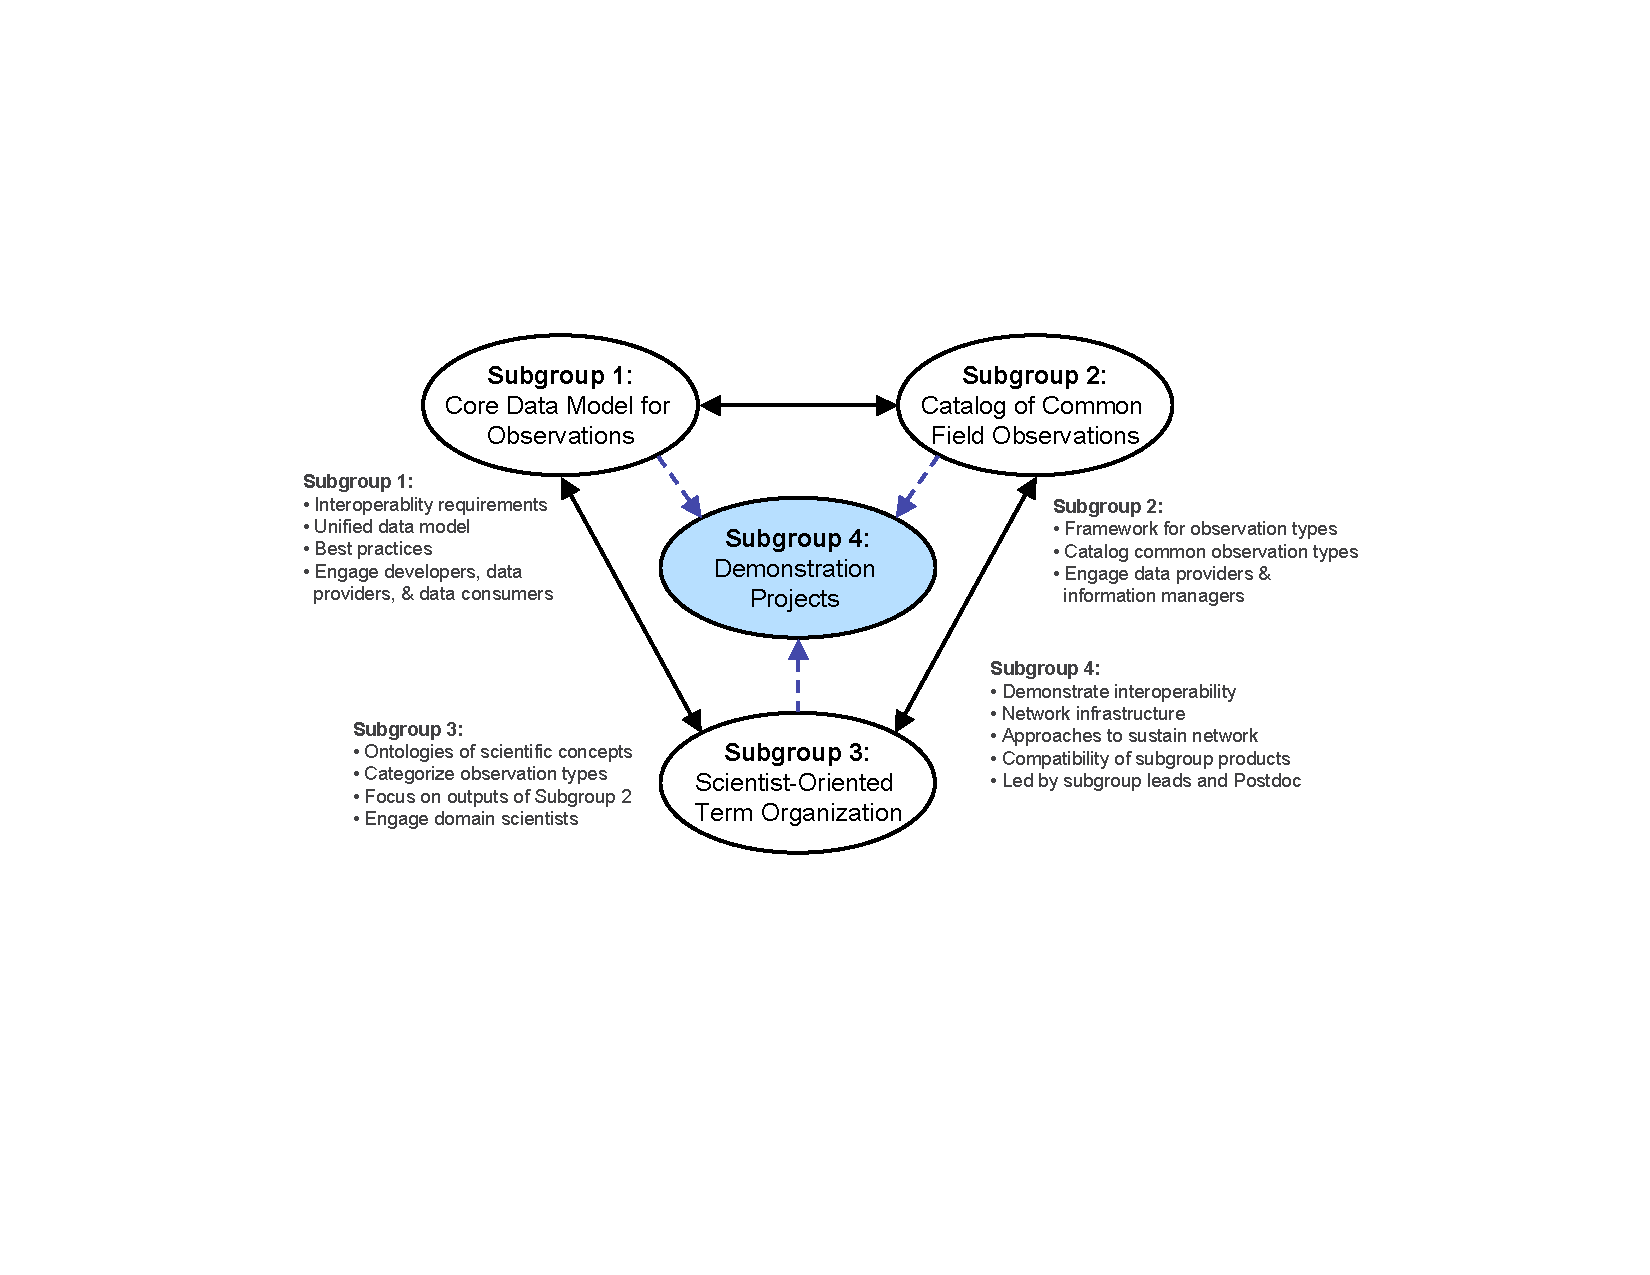
\includegraphics[scale=.4]{sonet-subgroups}
  \vspace{-8pt}
  \caption{{\small Primary \sonet\ working groups}}
  \label{fig:groups}
  \end{footnotesize}
\end{figure}

\mypara A key aspect of \sonet's approach has grown out of earlier
workshops, in which domain and information-management experts agreed
that the ``scientific observation'' provides a promising conceptual
linchpin for improved software interoperability and data integration
across disciplines. In the sense used here, a scientific observation
consists of the measurement of a characteristic of some entity, at a
given place and time.  The specifics of the entities and the
characteristics measured can be captured through emerging approaches
in semantic technologies, most promisingly via formal ontologies.

\begin{figure}[!h]
  \begin{footnotesize}
  \centering
  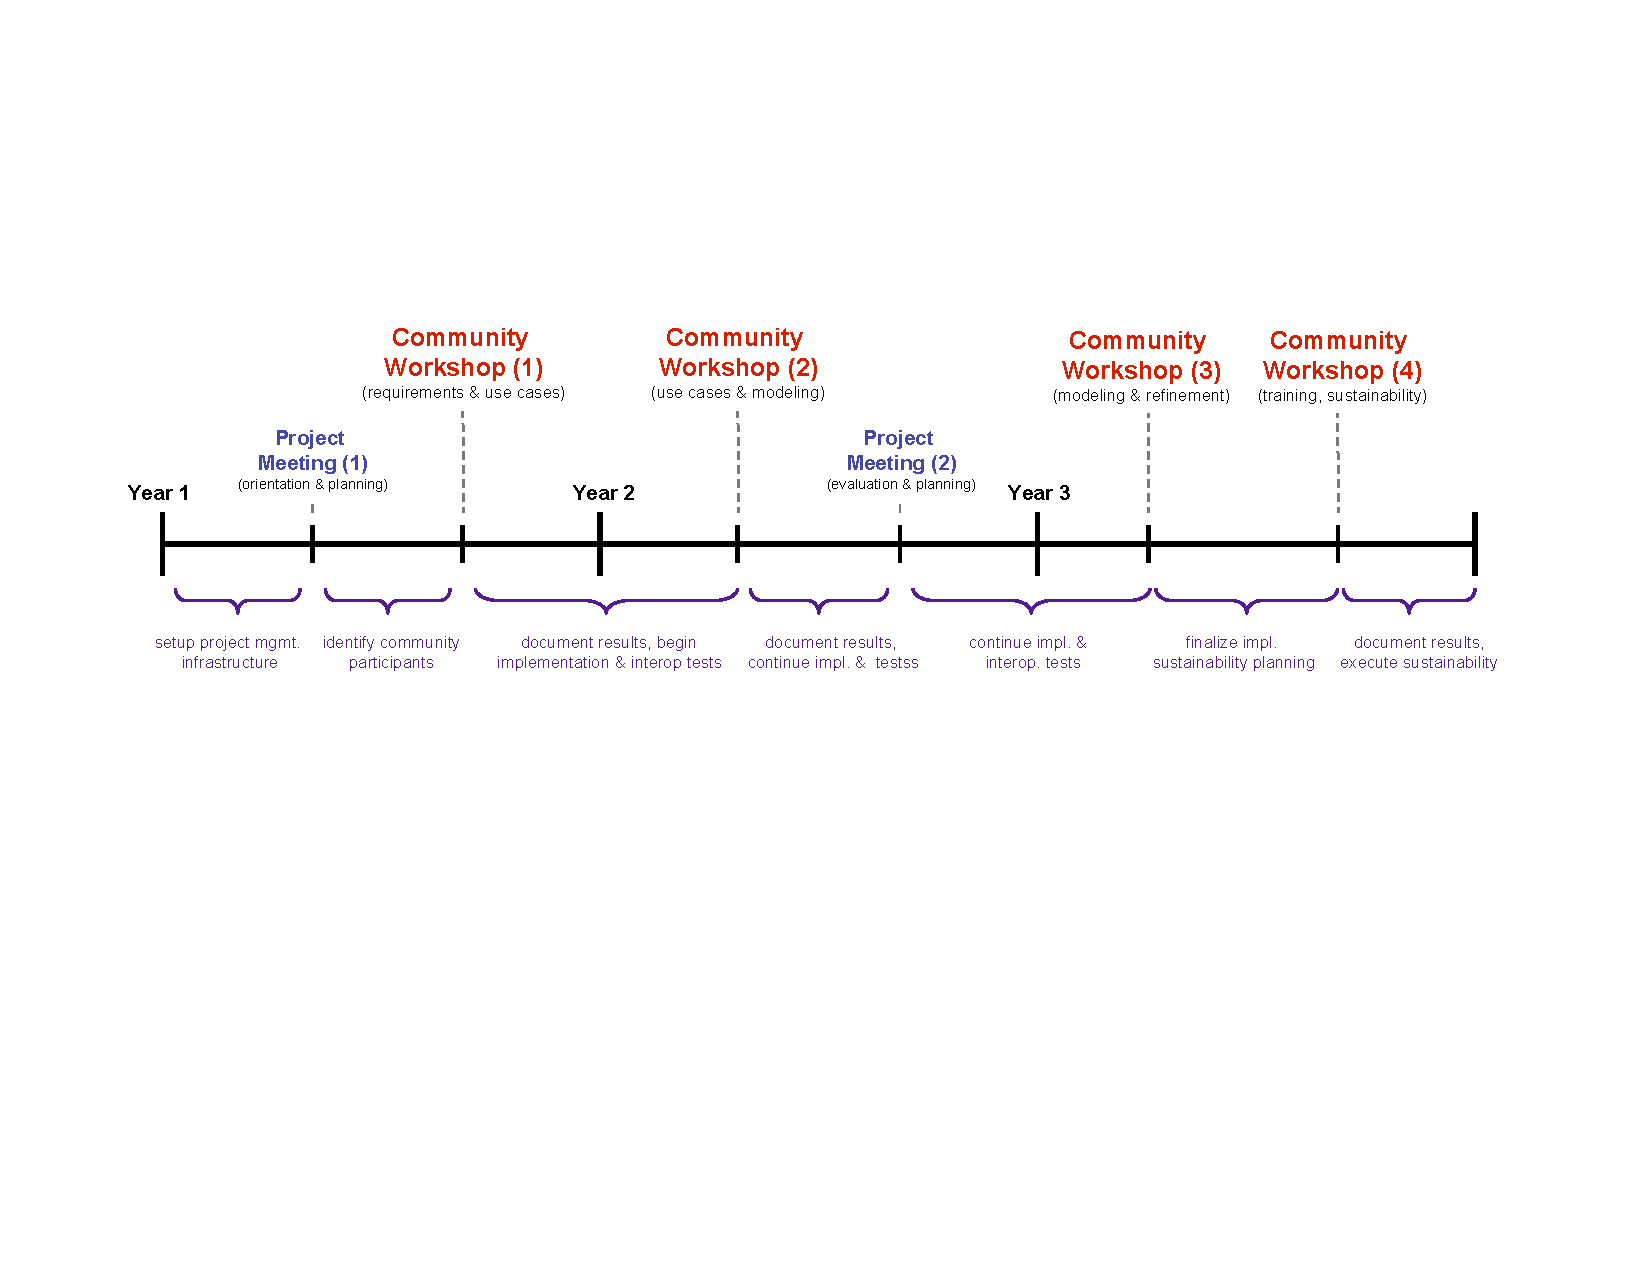
\includegraphics[scale=.35]{sonet-timeline}
  \vspace{-8pt}
  \caption{{\small Overview of \sonet\ workshops and activies}}
  \label{fig:timeline}
  \end{footnotesize}
\end{figure}

\mypara The \sonet\ effort provides resources to build a
cross-disciplinary community to refine and promote a unified approach
to modeling scientific data, through working groups
(\figref{fig:groups}) and a series of workshops
(\figref{fig:timeline}) and to begin the process of building
interoperable ontologies that capture the semantic nuances needed for
effectively communicating the meaning and interpretation of data to
specialists as well as scientists pursuing synthetic analyses.
Working groups together with network experts will also develop a
series of demonstration projects to illustrate the capabilities for
data interoperability.


\end{document}